\chapter{Teor\'ia} \justifying
Existen 2 tipos de ecuaciones diferenciales 2 tipos:
\begin{itemize}
    \item Lineales $y''+y=0$ (fáciles) $\Rightarrow P(D)y=0$. D operador derivada.
    \item No Lineales $y''+\sin(y)=0$.
\end{itemize}

Resolución: $y''+y=0 \Rightarrow P(D)y=0 \Rightarrow (D^2+1)=0 \Rightarrow p_c = x^2+1$ pol carac.

Si en vez del operador derivada $D$ elegimos el operador siguiente, $E$ tal que $E(y_n) = y_{n+1}$ y diferencia, $\nabla$ tal que $\nabla(y_n) = y_n - y_{n-1} = (I - E^{-1})y_n$, con la sucesión $\{y_n\}_{n=0}^{\infty}$ obtenemos ecuaciones en diferencias $P(E)y_n = 0$.

Casos según $p_c$:
\begin{enumerate}
    \item Raíces reales distintas
    \begin{enumerate}[noitemsep]
        \item $p_c = x-\lambda $
        \begin{itemize}[noitemsep]
            \item $y'-\lambda y = 0 \Rightarrow y(x) = c \, e^{\lambda x}$
            \item $y_{n+1}-\lambda y_n = 0 \Rightarrow y_n = c(\lambda)^n$
        \end{itemize}
        \item $p_c = (x-\lambda_1)\cdots(x-\lambda_n)$
        \begin{itemize}
            \item $y^{(n)} \dots + \lambda_1\cdots\lambda_n y = 0 \Rightarrow y(x) = c_1 e^{\lambda_1 x} + \dots + c_n e^{\lambda_n x}$
            \item $y_{n+n} \dots + \lambda_1\cdots\lambda_n y_n = 0 \Rightarrow y_n = c_1 \lambda_1^n + \dots + c_n \lambda_n^n$
        \end{itemize}
    \end{enumerate}
    \item Raíces dobles reales
    \begin{enumerate}[noitemsep]
        \item $p_c = (x-\lambda_1)^2$
        \begin{itemize}[noitemsep]
            \item $y''-2\lambda_1 y' + \lambda_1^2 y = 0 \Rightarrow y(x) = c_1 e^{\lambda_1 x} + c_2 x e^{\lambda_1 x}$
            \item  $y_{n+2}-2\lambda_1 y_{n+1} + \lambda_1^2 y_n = 0 \Rightarrow y_n = c_1 \lambda_1^n + c_2 n \lambda_1^n$
        \end{itemize}
        \item $p_c = (x-\lambda_1)^m $ 
        \begin{itemize}[noitemsep]
            \item $y^{(m)} + \dots + \lambda_1^m y = 0 \Rightarrow y(x) = c_1 e^{\lambda_1 x} + c_2 x e^{\lambda_1 x} + \dots + c_m x^{m-1} e^{\lambda_1 x}$
            \item $y_{m+n} +\dots + \lambda_1^m y_n = 0 \Rightarrow y_n = c_1 \lambda_1^n + c_2 n \lambda_1^n + \dots + c_m n^{m-1} \lambda_1^n$
        \end{itemize}
    \end{enumerate}
    \item Raíces complejas. $\varrho = \sqrt{a^2+b^2}$, $\theta = \arctan(b/a) $
    \begin{enumerate}[noitemsep]
        \item $p_c = x^2 -2ax + (a^2 + b^2) = (x-a+bi)(x-a-bi) \Rightarrow r_1=a+bi, \, r_2 = a-bi$
        \begin{itemize}[noitemsep]
            \item $y'' - 2ay' + (a^2 + b^2)y = 0$ 
            \begin{align*}
                  y(x) & = A e^{(a+bi)x} + B e^{(a-bi)x} = e^{ax} \left( A e^{ibx} + B e^{-ibx} \right)  \\  & = e^{ax} \left[ (A+B)\cos(bx) + i(A-B)\sin(bx) \right]  \\  & = e^{ax}(c_1 \cos(bx) + c_2 \sin(bx))
            \end{align*}
            \item $y_{n+2} - 2ay_{n+1} + (a^2 + b^2)y_n = 0$
            \begin{align*}
                y_n & = A r_1^n + B r_2^n = A(\varrho e^{i\theta})^n + B(\varrho e^{-i\theta})^n  \\  & = \varrho^n \left[ (A+B)\cos(\theta n) + i(A-B)\sin(\theta n) \right]   \\  & = \varrho^n(c_1 \cos(\theta n) + c_2 \sin(\theta n))
            \end{align*}
        \end{itemize}
        \item $p_c = (x-a+bi)^m (x-a-bi)^m$
        \begin{itemize}[noitemsep]
            \item $y^{(m)} + \cdots + b^{2m} y = 0 \Rightarrow$ \begin{align*}
                y(x) = e^{a x}& \Big[ c_1 \cos b x + c_2 \sin b x +  x(c_3 \cos b x + c_4 \sin b x) + \cdots + x^{m-1}(c_{2m-1} \cos b x + c_{2m} \sin b x)\Big] \\ 
                 = e^{a x} &  \sum_{k=0}^{m-1} x^k \left( c_{2k+1} \cos(b x) + c_{2k+2} \sin(b x) \right) 
            \end{align*}
            \item $y_{m+n} + \cdots + b^{2m} y_n = 0 \Rightarrow$ \begin{align*}
               y_n = \varrho^n &  \Big[ c_1 \cos \theta n + c_2 \sin \theta n +  n(c_3 \cos \theta n + c_4 \sin \theta n) +  \cdots + n^{m-1}(c_{2m-1} \cos \theta n + c_{2m} \sin \theta n) \Big] \\ =  \varrho^n & \sum_{k=0}^{m-1} n^k \left( c_{2k+1} \cos(\theta n) + c_{2k+2} \sin(\theta n) \right)            
            \end{align*} 
        \end{itemize}
    \end{enumerate}
\end{enumerate}

\section{Convergencia, estabilidad y consistencia}

\begin{defi}
    Un método numérico es una ecuación:
\begin{equation}
    \sum_{j=0}^k \alpha_j y_{n+j} = h \phi_f(y_{n+k}, \dots, y_n, x_n; h) \tag{2.4}
\end{equation}
donde el subíndice $f$ indica la dependencia de $\phi$ en $y_{n+k} \dots y_n, x_n$ por la función $f(x,y) = y'$.

Se imponen dos condiciones para que sea método:
\begin{equation}
\begin{aligned}
1. & \, \phi_{f=0}(y_{n+k}, \dots, y_n, x_n; h) \equiv 0, \\
2. & \, \displaystyle \|\phi_f(y_{n+k}, \dots, y_n, x_n, h) - \phi_f(y^*_{n+k}, \dots, y^*_n, x_n, h)\| \le M \sum_{j=0}^k \|y_{n+j} - y^*_{n+j}\|.
\end{aligned}
\tag{2.5}
\end{equation}
 siendo $M$ una constante, y 2) una consecuencia de la condición de Lipschitz para la existencia de soluciones (Teorema del Valor Medio).
\end{defi} 

\begin{defi}
    Un método es convergente si para todo problema de valor inicial se cumple
$$ \lim_{\substack{h \to 0 \\ x = a+nh}} y_n = y(x) $$
\end{defi} 

\begin{defi}
    El operador local de error truncado en $k$ es:
$$ \mathscr L = \sum_{j=0}^k \alpha_j y(x_{n+j}) - h \phi_f(y(x_{n+k}), \dots, y(x_n), x_n; h) = \mathcal{O}(h^p) \text{ al menos} $$
y mide la diferencia entre la solución real y la del método numérico.
\end{defi}

\begin{defi}
    Un método se dice consistente si para cualquier c.i.:
$$ \lim_{h \to 0} \frac{1}{h}\mathscr L = 0 $$
(consistente con el sistema de ecuaciones diferenciales).
\end{defi}

\begin{defi}
    Se define el primer polinomio caracter\'istico $\rho$ del método numérico como:
$$ \rho(\zeta) = \sum_{j=0}^k \alpha_j \zeta^j $$
\end{defi} 

\begin{prop} Un método es consistente si y solo si satisface:
\begin{enumerate}[itemsep=1em]
    \item $\rho(1) = 0$
    \item $\dfrac{\phi_f(y(x_n), \dots, y(x_n), x_n, 0)}{\rho'(1)} = f(x_n, y(x_n))$
\end{enumerate}
\end{prop}

\begin{defi}
    Dada $y'=f(x,y)$, $y(a)=\eta$, y una perturbación $\varepsilon$, $y^{*\prime}=f(x,y^*)+\varepsilon(x)$ $y^*(a)=\eta+\varepsilon$, decimos que un sistema es \textit{totalmente estable} si existe $S \ge 0$ t.q. $\forall x \in [a,b]$,
$$ ||y(x) - y^*(x)|| \le S \varepsilon$$
\end{defi} 
   
 \begin{defi}  
Sean $\{\delta_n, n=0, 1, \dots, N\}$ y $\{\delta_n^*, n=0, 1, \dots, N\}$ dos perturbaciones cualesquiera del sistema diferencial, y sean $\{z_n, n=0, 1, \dots, N\}$ y $\{z_n^*, n=0, 1, \dots, N\}$ las soluciones perturbadas resultantes. Entonces, si existen constantes $S$ y $h_0$ tales que, para todo $h \in (0, h_0]$:
   $$\vert{}\vert{}z_n - z_n^*\vert{}\vert{} \le S\varepsilon, \quad 0 \le n \le N$$siempre que:$$\vert{}\vert{}\delta_n - \delta_n^*\vert{}\vert{} \le \varepsilon, \quad 0 \le n \le N$$
se dice que un método es \textit{zero-stable}. 
\end{defi}

\begin{defi}[alternativa] Se dice que un método es \textit{zero-stable} si satisface la condición de la raíz (es decir, si todas las raíces de su primer polinomio característico tienen un módulo menor o igual a uno, y aquellas de módulo uno son simples).
\end{defi}

\begin{teo}
    [2.1] La condición necesaria y suficiente para que el método dado por (2.4) y (2.5) sea zero-estable es que satisfaga la condición de la raíz.
\end{teo}
\begin{teo}
    [2.2] Las condiciones necesarias y suficientes para que un método num\'erico sea convergente son que sea tanto consistente como zero-estable.
\end{teo} 

\begin{obs}
    Existen dos tipos de estabilidad, que vemos a continuaci\'on:
\begin{center}
\begin{tikzpicture}[xscale=1.2, yscale=1]
    % 1. Estable
    \node[anchor=west] at (0, 0) {\underline{Estable}};
    \draw (2.5, 0.2) .. controls (3.5, 0.4) and (4.5, -0.1) .. (5.5, 0.2) .. controls (6.5, 0.5) and (7.5, 0.1) .. (8.5, 0.2);
    \draw (2.5,-0.2) .. controls (3.5, 0.0) and (4.5,-0.5) .. (5.5,-0.2) .. controls (6.5, 0.1) and (7.5,-0.3) .. (8.5,-0.2);
    \draw (8.5, 0.6) -- (8.5, -0.6);
    \node[anchor=west] at (9.0, 0) {$S_\varepsilon = cte.$};
    \fill (2.5, 0.2) circle (1.5pt);
    \fill (2.5, -0.2) circle (1.5pt);

    % 2. Asintóticamente estable
    \node[anchor=west, align=left] at (0, -2.5) {\underline{Asintóticamente}\\\quad \underline{estable}};
    \fill (3.5, -2.0) circle (1.5pt);
    \fill (3.5, -3.0) circle (1.5pt);
    \draw (3.5, -2.0) to[out=0, in=180] (8.5, -2.4);
    \draw (3.5, -3.0) to[out=0, in=180] (8.5, -2.6);
    \node[anchor=west] at (9.0, -2.5) {$S_\varepsilon \xrightarrow{t \to \infty} 0$};

    % 3. Inestable
    \node[anchor=west] at (0, -5.5) {\underline{Inestable}};
    \node[anchor=east] at (3.4, -5.5) {$x_0 + \varepsilon$};
    \fill (3.5, -5.5) circle (1.5pt);
    \node[anchor=east] at (3.4, -6.0) {$x_0$};
    \fill (3.5, -6.0) circle (1.5pt);
    \draw (3.5, -5.5) to[out=0, in=200] (8.5, -4.0);
    \draw (3.5, -6.0) to[out=0, in=160] (8.5, -7.0);
    \node[anchor=west] at (9.0, -5.5) {$S_\varepsilon \longrightarrow \infty$};
\end{tikzpicture}
\end{center}
\end{obs}

\begin{ejem}
    En la ecuaci\'on $y'=\lambda y$ con las condiciones iniciales $y_o$ y la perturbada $y_o+\varepsilon$, se tienen las soluciones $y(x) = y_o e^{\lambda x}, \, y(x) = (y_o + \varepsilon) e^{\lambda x}$, de forma que 
    $$\begin{array}{cc}
         y_o + e^{\lambda x}   \\
        - \,  (y_o + \varepsilon) e^{\lambda x} \\ \hline
        \varepsilon e^{\lambda x} 
    \end{array}\Rightarrow \lim_{\lambda \to \infty} \varepsilon e^{\lambda x}  = 0 \iff \lambda \leq 0$$
    siendo $\lambda$ claramente la ra\'iz de $p_c = x-\lambda$. As\'i, si $\lambda < 0$ es asint\'oticamente estable, si $\lambda=0$ es estable y si $\lambda> 0$ es inestable.
\end{ejem}

\section{Análisis de la estabilidad en función de las raíces $r_i$ del polinomio característico}
\subsection*{Ecuaciones diferenciales}
\begin{itemize}
    \item \textbf{Raíces reales simples}
    \begin{itemize}
        \item $r_i < 0 \implies$ Asintóticamente estable.
        \item $r_i = 0 \implies$ Estable.
        \item $r_i > 0 \implies$ Inestable.
    \end{itemize}
    
    \item \textbf{Raíces complejas simples}
    \begin{itemize}        
        \item $a=\Re(r_i) < 0 \implies$ Asint\'oticamente estable.
        \item $a=\Re(r_i) = 0 \implies$ Estable.
        \item $a=\Re(r_i) > 0 \implies$ Inestable.
    \end{itemize}
    
    \item \textbf{Raíces dobles o múltiples (reales o complejas)}
    \begin{itemize}
        \item Siempre inestables (la solución se multiplica por la variable temporal).
    \end{itemize}
\end{itemize}

\subsection*{Ecuaciones en diferencias}
\begin{itemize}
    \item \textbf{Raíces simples (reales o complejas)}
    \begin{itemize}
        \item $|r_i| < 1 \implies$ Asintóticamente estable.
        \item $|r_i| = 1 \implies$ Estable.
        \item $|r_i| > 1 \implies$ Inestable.
    \end{itemize}
    
    \item \textbf{Raíces dobles o múltiples}
    \begin{itemize}
        \item $|r_i| < 1 \implies$ Asintóticamente estable.
        \item $|r_i| = 1 \implies$ Inestable.
        \item $|r_i| > 1 \implies$ Inestable.
    \end{itemize}
\end{itemize}
\begin{obs}
    Para poder utilizar estos m\'etodos num\'ericos en ecuaciones de orden mayor que 1 necesitamos pasarlas a sistemas aut\'onomos, de forma que ya $y_i'=f(x,y_i)$, es decir, que $Y'=F(Y)$ siendo $Y = (y_1, \ldots, y_n)$. 
\end{obs}

\section{M\'etodos Runge-Kutta}
\begin{defi}
    El m\'etodo Runge-Kutta de $s$-etapas general para el problema
    $$y' = f(x,y) \qquad y(a)=\eta \qquad f:\bb R \times \bb R^m \longrightarrow \bb R^m$$
    se define como
    $$y_{n+1} = y_n + h \sum_{i=1}^s b_i k_i$$
    donde 
    $$k_i = f \left( x_n +c_i h, \, y_n + h \sum_{j=1}^s a_{ij} k_j \right)\qquad i=1,2,\ldots, s$$
\end{defi}

Debemos asumir siempre que se cumple que 
$$c_i = \sum_{j=1}^s a_{ij} \qquad i=1,2,\ldots, s$$

Es conveniente presentar los coeficientes como una \textit{matriz de Butcher}
$$\begin{array}{c|cccc}
     c_1 & a_{11} & a_{12} & \cdots &  a_{1s} \\
     c_2 & a_{21} & a_{22} & \cdots &  a_{2s} \\ 
     \vdots & \vdots & &  & \vdots \\ 
     c_s & a_{s1} & a_{s2} & \cdots &  a_{ss} \\ \hline
     & b_1 & b_2 & \cdots & b_s
\end{array}$$
Definimos los vectores $s$-dimensionales $c$ y $b$ y la matriz $s\times s$ $A$ como
$$c=[c_1, c_2, \ldots, c_s]^t \quad b = [b_1, b_2, \ldots, b_s]^t \quad A = [a_{ij}]$$
Nótese que, según la condici\'on de $c_i$, las componentes de $c$ son las sumas de las filas de $A$. Claramente, un método de Runge-Kutta de $s$ etapas queda completamente especificado por su tabla de Butcher:
\begin{equation*}
    \begin{array}{c|c}
        c & A \\
        \hline
        & b^T
    \end{array}
\end{equation*}
Una forma alternativa de la definici\'on del m\'etodo, que en algunos contextos resulta más cómoda, es
$$ y_{n+1} = y_n + h \sum_{i=1}^{s} b_i f(x_n + c_i h, Y_i)$$
donde
$$ Y_i = y_n + h \sum_{j=1}^{s} a_{ij} f(x_n + c_j h, Y_j) \qquad i = 1, 2, \dots, s$$
Se puede ver que ambas formas son equivalentes si hacemos la interpretación
$$k_i = f(x_n + c_i h, Y_i) \qquad i = 1, 2, \dots, s$$

Al sustituir $$k = 1, \quad \alpha_1 = 1, \quad \alpha_0 = -1, \quad \phi_f(y_n, x_n; h) = \sum_{i=1}^{s} b_i k_i$$
vemos que los m\'etodos num\'ericos antes definidos contienen los métodos de Runge-Kutta.

Recordando que las condiciones necesarias y suficientes para que un m\'etodo sea consistente son
$$\sum_{j=0}^{k} \alpha_j = 0, \qquad \frac{\phi_f(y(x_n), y(x_n), \dots, y(x_n), x_n; 0)}{\sum_{j=0}^{k} j \alpha_j} = f(x_n, y(x_n))$$
Aplicando estas condiciones a los m\'etodos Runge-Kutta vemos que la condición necesaria y suficiente para que un método general sea consistente es
$$\phi_f(y(x_n), x_n; 0) = f(x_n, y(x_n)) \iff \sum_{i=1}^{s} b_i = 1$$

Así pues, el método de Runge-Kutta explícito de 3 etapas se puede escribir como   
$$ \begin{aligned}     y_{n+1} &= y_n + h(b_1 k_1 + b_2 k_2 + b_3 k_3) \\     k_1 &= f(x_n, y_n) \\     k_2 &= f(x_n + h c_2, y_n + h c_2 k_1) \\     k_3 &= f(x_n + h c_3, y_n + h(c_3 - a_{32})k_1 + h a_{32} k_2) \end{aligned}$$

Asumimos que $f(x, y)$ es suficientemente diferenciable e introducimos la notación abreviada   
$$f := f(x, y), \quad f_x := \frac{\partial f(x,y)}{\partial x}, \quad f_{xx} := \frac{\partial^2 f(x,y)}{\partial x^2}, \quad f_{xy} (\equiv f_{yx}) := \frac{\partial^2 f(x,y)}{\partial x \partial y}$$ 
etc., todo evaluado en el punto $(x_n, y(x_n))$. Al expandir $y(x_{n+1})$ alrededor de $x_n$ como una serie de Taylor, tenemos:
$$y(x_{n+1}) = y(x_n) + h y^{(1)}(x_n) + \frac{1}{2}h^2 y^{(2)}(x_n) + \frac{1}{6}h^3 y^{(3)}(x_n) + O(h^4).$$
Ahora:
$$\left\{ \begin{aligned}     y^{(1)}(x_n) &= f \\     y^{(2)}(x_n) &= f_x + f_y y' = f_x + f f_y \\     y^{(3)}(x_n) &= f_{xx} + 2f f_{xy} + f^2 f_{yy} + f_y(f_x + f f_y) \end{aligned} \right.$$
Abreviemos la notación nuevamente definiendo:
$$F := f_x + f f_y, \quad G := f_{xx} + 2f f_{xy} + f^2 f_{yy}$$
de modo que podemos escribir la expansión para $y(x_{n+1})$ como   
$$y(x_{n+1}) = y(x_n) + hf + \frac{1}{2}h^2 F + \frac{1}{6}h^3 (F f_y + G) + O(h^4)$$
Expandiendo el término $k_1 = f$ y sustituyendo:
$$k_2 = f + h c_2 F + \frac{1}{2}h^2 c_2^2 G + O(h^3).$$
Y análogamente para $k_3$:
$$\begin{aligned} k_3 = f &+ h \{c_3 f_x + [(c_3 - a_{32})k_1 + a_{32}k_2]f_y\} \\ &+ \frac{1}{2}h^2 \{c_3^2 f_{xx} + 2c_3 [(c_3 - a_{32})k_1 + a_{32}k_2] f_{xy} + [(c_3 - a_{32})k_1 + a_{32}k_2]^2 f_{yy}\} + O(h^3). \end{aligned}$$

\begin{ejems} \, 
    \begin{itemize}
        \item Euler expl\'icito: $y_{n+1} = y_n + h f_n \qquad f_n = f(x_n,\, y_n)$
        \item Euler impl\'icito: $y_{n+1} = y_n + h f_{n+1} \qquad f_{n+1} = \phi_f $
        \item Runge-Kutta: $y_{n+1} = y_n + h(b_1 f_n + b_2 f_{n+1}) $
        
        \hspace{1.5cm} $y_{n+1} = y_n + h(b_1 k_1 + b_2 k_2) $ donde $k_1 = f(x_n,\, y_n), \, k_2 = f(x_n,\, y_n+h \cdot k_1)$
        \item Multipaso: $y_{n+1} = y_n + h \left( f_n + \frac{1}{2} \nabla f_n  + \frac{1}{4} \underbrace{\nabla^2 f_n}_{\nabla f_n-\nabla f_{n-1}} \right)$
    \end{itemize}
\end{ejems}

\begin{defi}
    Se define el orden de un m\'etodo RK como el $p$ tal que el Error de Truncamiento Local sea:
    $$\mathscr L = y(x_n +h) - y(x_n) - \sum b_i k_i = F(y_1) h^{p+1} + \mc O (h^{p+2})$$
\end{defi}
(Parcial I)
\newpage 

% ---------------------------------------------------------
% SECCIÓN REORGANIZADA: TEORÍA DE BUTCHER
% ---------------------------------------------------------

\section{Teoría de Butcher: Derivadas de Fréchet, \'arboles y correspondencia} 
\subsection{Introducci\'on} 
%Las ideas que estamos a punto de describir se remontan a un artículo de Merson (1957), pero su desarrollo en una teoría importante se debe a J. C. Butcher, en una larga serie de artículos que comenzaron a mediados de la década de 1960. El lector que desee ver una descripción completa de la teoría puede consultar el libro de Butcher (1987) que, dicho sea de paso, contiene la bibliografía disponible más completa sobre el tema de los métodos numéricos para ecuaciones diferenciales ordinarias, con unas 2000 entradas. En las secciones siguientes presentaremos solo una versión simplificada de la teoría, con el objetivo de permitir al lector utilizar la teoría para establecer las condiciones de orden (y la estructura del error de truncamiento local) y apreciar algunas de las consecuencias. En particular, no daremos ninguna prueba de los teoremas involucrados, y nuestro tratamiento de los aspectos algebraicos no será riguroso (¡posiblemente hasta el punto de ofender a algunos lectores!).
\footnote{Lambert p. 157-162}Recordemos que, si bien hay una pérdida de generalidad al asumir que el problema de valor inicial \textit{escalar} es autónomo, no hay tal pérdida en el caso de un problema que involucra un sistema de ecuaciones diferenciales ordinarias. Ahora estamos tratando con sistemas, y se logra una simplificación útil asumiendo la forma autónoma
\begin{equation}
y' = f(y), \quad y(a) = \eta, \qquad f : \mathbb{R}^m \to \mathbb{R}^m, \quad m > 1 \tag{5.22}
\end{equation}
Comencemos por ver en qué dificultades nos metemos al tratar de adaptar el enfoque de la sección anterior al caso de sistemas. El primer problema con el que nos encontramos es la contraparte de (5.14), donde necesitamos expresar las derivadas totales de $y$ en términos de $f$ y sus derivadas parciales. Para el caso autónomo \textit{escalar} (5.14) se lee
\begin{equation}
y^{(1)} = f, \quad y^{(2)} = f_y f, \quad y^{(3)} = f_{yy} f^2 + f_y^2 f. \tag{5.23}
\end{equation}
¿Cuáles son las expresiones correspondientes cuando $y, f \in \mathbb{R}^m$? Para mantener las cosas simples, consideremos el caso $m = 2$, de modo que $y = [\,\!^1y, \!^2y]^T$, $f = [\, \!^1f, \!^2f]^T$. Introduciendo la notación
\[
\!^i f_j := \frac{\partial (\, \!^i f)}{\partial (\, \!^j y)}, \quad \!^i f_{jk} := \frac{\partial^2 (\, \!^i f)}{\partial (\, \!^j y) \partial (\, \!^k y)} \quad \text{etc.}
\]
tenemos $\!^1 y^{(1)} = \!^1 f$, $\!^2 y^{(1)} = \!^2 f$, de donde encontramos al derivar que
\begin{equation*}
\!^1 y^{(2)} = \!^1 f_1 (\, \!^1 f) + \!^1 f_2 (\, \!^2 f), \quad \!^2 y^{(2)} = \!^2 f_1 (\, \!^1 f) + \!^2 f_2 (\, \!^2 f)
\end{equation*}
o
\begin{equation}
y^{(2)} = \begin{pmatrix} \!^1 f_1 & \!^1 f_2 \\ \!^2 f_1 & \!^2 f_2 \end{pmatrix} f \tag{5.24}
\end{equation}
y
\begin{equation}
\left.
\begin{aligned}
\!^1 y^{(3)} &= \!^1 f_{11} (\, \!^1 f)^2 + \!^1 f_{12} (\, \!^1 f)(\, \!^2 f) + \!^1 f_1 \left[\, \!^1 f_1 (\, \!^1 f) + \!^1 f_2 (\, \!^2 f)\right] \\
&\quad + \!^1 f_{21} (\, \!^2 f)(\, \!^1 f) + \!^1 f_{22} (\, \!^2 f)^2 + \!^1 f_2 \left[\, \!^2 f_1 (\, \!^1 f) + \!^2 f_2 (\, \!^2 f)\right] \\
\!^2 y^{(3)} &= \!^2 f_{11} (\, \!^1 f)^2 + \!^2 f_{12} (\, \!^1 f)(^2 f) +\!^2 f_1 \left[\, \!^1 f_1 (\, \!^1 f) + \!^1 f_2 (^2 f)\right] \\
&\quad +\!^2 f_{21} (^2 f)(\!^1 f) +\!^2 f_{22} (^2 f)^2 +\!^2 f_2 \left[^2 f_1 (\, \!^1 f) +\!^2 f_2 (^2 f)\right]
\end{aligned}
\right\} \tag{5.25}
\end{equation}

Notemos que (5.24) se puede escribir como $y^{(2)} = \partial f / (\partial y) f$, donde $\partial f / \partial y$ es la matriz Jacobiana, una generalización natural de la segunda de (5.23). Por el contrario, (5.25) no se puede escribir en forma de matriz/vector, y no se parece en nada a una generalización de la última de (5.23).

Claramente no podemos seguir así para evaluar derivadas aún más altas (y todavía no hemos considerado el caso de un $m$ general). Una mejor notación es esencial, y de hecho se necesita más que una notación; necesitamos descubrir una \textit{estructura} para estas derivadas superiores. (En cuanto a la cuestión de la notación, se debe advertir al lector que en las siguientes secciones cambiaremos (y simplificaremos) continuamente la notación; la pauta será que tan pronto como nos familiaricemos con una notación particular, intentaremos simplificarla aún más).


\subsection{Derivadas de Fréchet y diferenciales elementales}

Dada la notación para un sistema de ecuaciones diferenciales autónomo $y' = f(y)$, definimos el vector de variables $y = [\, \!^1y, \!^2y, \dots, \!^my]^T$ y el campo vectorial $f = [\, \!^1f, \!^2f, \dots, \!^mf]^T$.
Definimos las derivadas parciales con la notación por componentes:
$$ {\!^i}f_j = \frac{\partial \, \!^if}{\partial \, \!^jy}, \quad {\!^i}f_{jk} = \frac{\partial^2 \, {\!^i}f}{\partial \, \!^jy \, \partial \, \!^ky} $$

\begin{defi}[$M$-ésima Derivada de Fréchet]
Sea $z, f(z) \in \mathbb{R}^m$. La $M$-ésima derivada de Fréchet de $f$, denotada por $f^{(M)}(z)$, es un operador multilineal sobre $\mathbb{R}^m \times \dots \times \mathbb{R}^m$ ($M$ veces), lineal en cada uno de sus operandos, cuya expresión por componentes es:
\[
f^{(M)}(z)(K_1, K_2, \dots, K_M) = \sum_{i=1}^{m} \sum_{j_1=1}^{m} \dots \sum_{j_M=1}^{m} {^i}f_{j_1 j_2 \dots j_M} \left(^{j_1}K_1\right) \left(^{j_2}K_2\right) \dots \left(^{j_M}K_M\right) e_i
\]
Donde $K_t = \left[ \, {\!^1}K_t, \dots, {\!^m}K_t \right]^T \in \mathbb{R}^m$ son los vectores operandos, ${\!^i}f_{j_1 j_2 \dots j_M}$ son las derivadas parciales de orden $M$, y $e_i$ es el $i$-ésimo vector canónico en $\mathbb{R}^m$.
\end{defi}

\subsubsection*{Desarrollo de las derivadas totales hasta orden 3}
Mediante la notación de Fréchet con llaves $\{\}$, las derivadas totales de la solución exacta $y^{(q)}$ se descomponen de forma limpia como combinaciones lineales de \textit{diferenciales elementales}:

\begin{itemize}
    \item \textbf{Orden 1:} $y^{(1)} = f$
    \item \textbf{Orden 2:} 
    $$y^{(2)} = \frac{d}{dt} y^{(1)} = \frac{\partial f}{\partial y} \frac{dy}{dt} = \frac{\partial f}{\partial y} f = f^{(1)}(f) = \{f\}$$
    (Corresponde a la matriz Jacobiana multiplicada por $f$)
    \item \textbf{Orden 3:} 
    Aplicando la regla de la cadena multivariable:
    $$y^{(3)} = \frac{d}{dt} y^{(2)} = f^{(2)}(f, f) + f^{(1)}(f^{(1)}(f)) = \{f^2\} + \{f\}_2$$
    Donde el término bilineal $f^{(2)}(k_1, k_2)$ se construye con las matrices Hessianas (derivadas segundas).
\end{itemize}


Pongamos ahora $m = 2$, y veamos si podemos interpretar los resultados (5.24) y (5.25) de la sección anterior en términos de derivadas de Fréchet.

\textbf{Caso $M = 1$}
\begin{align}
f^{(1)}(z)(K_1) &= \sum_{i=1}^2 \sum_{j_1=1}^2 {}^i f_{j_1} ({}^{j_1} K_1) e_i = \begin{bmatrix} \!^1 f_1 (\, \!^1 K_1) + \!^1 f_2 (^2 K_1) \\\!^2 f_1 (\, \!^1 K_1) +\!^2 f_2 (^2 K_1) \end{bmatrix} \tag{5.28}
\end{align}
donde
\[
^i f_1 = \frac{\partial (^i f)}{\partial (\, \!^1 z)}, \quad ^i f_2 = \frac{\partial (^i f)}{\partial (^2 z)}, \quad i = 1, 2.
\]

Ahora reemplazamos $z$ por $y$, y $K_1$ por $f$ (notando que los cuatro son vectores de dimensión 2). La ecuación (5.28) ahora se lee
\begin{equation}
f^{(1)}(y)(f(y)) = \begin{bmatrix} \!^1 f_1 (\, \!^1 f) + \!^1 f_2 (^2 f) \\\!^2 f_1 (\, \!^1 f) +\!^2 f_2 (^2 f) \end{bmatrix} = y^{(2)} \tag{5.29}
\end{equation}
por (5.24). En el contexto de la derivación de los métodos de Runge-Kutta, realmente no necesitamos que se nos diga que las derivadas parciales de $f$ se deben tomar con respecto al componente de $y$ (¿qué más hay?), de modo que podemos acortar la notación en (5.29) a
\begin{equation}
y^{(2)} = f^{(1)}(f). \tag{5.30}
\end{equation}
Así, la segunda derivada de $y$ es la primera derivada de Fréchet de $f$ operando sobre $f$; de (5.24) vemos que esto es equivalente a decir que la segunda derivada de $y$ es el Jacobiano de $f$ operando sobre $f$.

\textbf{Caso $M = 2$}
\begin{align*}
f^{(2)}(z)(K_1, K_2) &= \sum_{i=1}^2 \sum_{j_1=1}^2 \sum_{j_2=1}^2 \,^i f_{j_1 j_2} ({}^{j_1} K_1) ({}^{j_2} K_2) e_i \\
&= \begin{bmatrix} \!^1 f_{11} (\, \!^1 K_1)(\!^1 K_2) + \!^1 f_{12} (\, \!^1 K_1)(^2 K_2) + \!^1 f_{21} (^2 K_1)(\!^1 K_2) + \!^1 f_{22} (^2 K_1)(^2 K_2) \\ \!^2 f_{11} (\, \!^1 K_1)(\,\!^1 K_2) + \!^2 f_{12} (\, \!^1 K_1)(^2 K_2) + \!^2 f_{21} (\,\!^2 K_1)(\!^1 K_2) + \!^2 f_{22} (^2 K_1)(^2 K_2) \end{bmatrix}
\end{align*}
Reemplazamos $z$ por $y$ y ponemos $K_1 = K_2 = f$ para obtener
\begin{equation}
f^{(2)}(y)(f(y), f(y)) = \begin{bmatrix} \!^1 f_{11} (\, \!^1 f)^2 + 2(\,\!^1 f_{12})(\,\!^1 f)(^2 f) + \!^1 f_{22} (^2 f)^2 \\ \!^2 f_{11} (\, \!^1 f)^2 + 2(\,^2 f_{12})(\,\!^1 f)(^2 f) + \!^2 f_{22} (^2 f)^2 \end{bmatrix} \tag{5.31}
\end{equation}
donde la notación del lado izquierdo indica que las derivadas parciales son con respecto a los componentes de $y$, no de $z$. Al comparar con (5.25), vemos que el lado derecho de (5.31) representa algunos, pero no todos, de los términos del lado derecho de (5.25), y que obtenemos $y^{(3)}$ sumando al lado derecho de (5.31) el vector
\begin{equation}
\begin{bmatrix} \!^1 f_1 [\, \!^1 f_1 (\, \!^1 f) + \!^1 f_2 (^2 f)] + \!^1 f_2 [^2 f_1 (\, \!^1 f) + \!^2 f_2 (^2 f)] \\ \!^2 f_1 [\, \!^1 f_1 (\, \!^1 f) + \!^1 f_2 (^2 f)] + \!^2 f_2 [^2 f_1 (\, \!^1 f) + \!^2 f_2 (^2 f)] \end{bmatrix} \tag{5.32}
\end{equation}

Ahora bien, si en (5.29) reemplazamos el operando $f(y)$ por el operando $f^{(1)}(y)(f(y))$ (dado por la propia (5.29)), el resultado es precisamente (5.32). Por tanto, acortando la notación como en (5.30), (5.25) se puede escribir como
\begin{equation}
y^{(3)} = f^{(2)}(f, f) + f^{(1)}(f^{(1)}(f)) \tag{5.33}
\end{equation}
Comparando esto con la última de (5.23) (el resultado correspondiente para el caso escalar) vemos que hemos logrado una generalización que parece natural; es sencillo demostrar que cuando $m = 1$, $f^{(2)}(f, f)$ se reduce a $f_{yy} f^2$ y $f^{(1)}(f^{(1)}(f))$ a $f_y^2 f$.

Por supuesto, hemos probado los resultados (5.30) y (5.33) sólo para el caso $m = 2$, pero no es difícil ver que se cumplirán para todo $m$. Así, hemos visto que $y^{(2)}$ es una única derivada de Fréchet de orden 1 y que $y^{(3)}$ es una combinación lineal de derivadas de Fréchet de órdenes 1 y 2. En general, $y^{(p)}$ resulta ser una combinación lineal de derivadas de Fréchet de órdenes hasta $p - 1$. Los componentes en tales combinaciones lineales se llaman \textit{diferenciales elementales}; son las contrapartes para sistemas de términos como $F=f_x+ff_y$ y $G=f_{xx}+2ff_{xy}+f^2 f_{yy}$  para problemas escalares, y son los bloques de construcción naturales para los métodos de Runge-Kutta. Se definen recursivamente de la siguiente manera.d
\begin{defi} Los \textit{diferenciales elementales} $F_s : \mathbb{R}^m \to \mathbb{R}^m$ de $f$ y su orden se definen recursivamente por
\begin{itemize}
 \item [(i)] $f$ es el único diferencial elemental de orden 1, y 
 \item [(ii)] si $F_s, s = 1, 2, \dots, M$ son diferenciales elementales de órdenes $r_s$ respectivamente, entonces la derivada de Fréchet
\begin{equation}
f^{(M)}(F_1, F_2, \dots, F_M) \tag{5.34}
\end{equation}
es un diferencial elemental de orden
\begin{equation}
1 + \sum_{s=1}^M r_s. \tag{5.35}
\end{equation}
\end{itemize}
\end{defi}
El análisis tradicional del error mediante la expansión en series de Taylor multivariable se vuelve inmanejable para órdenes superiores a 3 en sistemas de ecuaciones. La Teoría de Butcher introduce una notación matemática y gráfica que simplifica drásticamente este proceso mediante el uso de derivadas de Fréchet y su correspondencia biunívoca con árboles enraizados.
















\subsection{Árboles enraizados y representación visual}

En la teoría de Runge-Kutta, para estructurar estas combinaciones algebraicas, se utiliza la teoría de grafos. Para cada uno de estos árboles elementales $t$, se calculan analíticamente tres parámetros clave
\begin{enumerate}
    \item \textbf{Orden $r(t)$:} Número total de nodos del árbol.
    \item \textbf{Simetría $\sigma(t)$:} Número de automorfismos estructurales del árbol.
    \item \textbf{Densidad $\gamma(t)$:} Parámetro fundamental que define el coeficiente exacto de la serie de Taylor ($1/\gamma(t)$). Se calcula multiplicando el número de nodos del árbol por las densidades de los subárboles que cuelgan de su raíz.
\end{enumerate}

\begin{defi} El \textbf{orden} $r(t)$, la \textbf{simetría} $\sigma(t)$ y la \textbf{densidad} $\gamma(t)$ de un árbol $t$ se definen mediante el caso base para el nodo simple:
\begin{equation*}
    r(\tau) = \sigma(\tau) = \gamma(\tau) = 1,
\end{equation*}
y de forma recursiva para un árbol compuesto por subramas $[t_1^{n_1} t_2^{n_2} \dots]$:
\begin{align*}
    r([t_1^{n_1} t_2^{n_2} \dots]) &= 1 + n_1 r(t_1) + n_2 r(t_2) + \dots \\
    \sigma([t_1^{n_1} t_2^{n_2} \dots]) &= n_1! \, n_2! \dots (\sigma(t_1))^{n_1} (\sigma(t_2))^{n_2} \dots \\
    \gamma([t_1^{n_1} t_2^{n_2} \dots]) &= r([t_1^{n_1} t_2^{n_2} \dots]) (\gamma(t_1))^{n_1} (\gamma(t_2))^{n_2} \dots
\end{align*}

Sea $\alpha(t)$ el número de formas esencialmente distintas de etiquetar los nodos del árbol $t$ con los números enteros $1, 2, \dots, r(t)$ de modo que las etiquetas aumenten a lo largo de cada arco saliente
\begin{equation*}
    \alpha(t) = \frac{r(t)!}{\sigma(t) \gamma(t)}
\end{equation*}
\end{defi}
\begin{obs}
    Lo que se entiende por ``esencialmente diferente'' se ilustra en los siguientes ejemplos:
\[
t_1 = [\tau^3] = \vcenter{\hbox{\begin{forest}
  for tree={grow=north, circle, fill=black, inner sep=1pt, minimum size=2.5pt, l sep=10pt, s sep=8pt}
  [ [ ] [ ] [ ] ]
\end{forest}}} . \quad \text{Entonces} \quad 
\vcenter{\hbox{\begin{forest}
  for tree={grow=north, circle, fill=black, inner sep=1pt, minimum size=2.5pt, l sep=10pt, s sep=8pt}
  [ , label=below:{\tiny 1} [ , label=above:{\tiny 2} ] [ , label=above:{\tiny 3} ] [ , label=above:{\tiny 4} ] ]
\end{forest}}} \quad \text{y} \quad 
\vcenter{\hbox{\begin{forest}
  for tree={grow=north, circle, fill=black, inner sep=1pt, minimum size=2.5pt, l sep=10pt, s sep=8pt}
  [ , label=below:{\tiny 1} [ , label=above:{\tiny 4} ] [ , label=above:{\tiny 2} ] [ , label=above:{\tiny 3} ] ]
\end{forest}}}
\]
etc. no se consideran etiquetados esencialmente diferentes, y $\alpha(t_1) = 1$.
\[
t_2 = [\tau[\tau]] = \vcenter{\hbox{\begin{forest}
  for tree={grow=north, circle, fill=black, inner sep=1pt, minimum size=2.5pt, l sep=10pt, s sep=8pt}
  [ [ ] [ [ ] ] ]
\end{forest}}} \, . \quad \text{Entonces} \quad 
\vcenter{\hbox{\begin{forest}
  for tree={grow=north, circle, fill=black, inner sep=1pt, minimum size=2.5pt, l sep=10pt, s sep=8pt}
  [ , label=below:{\tiny 1} [ , label=above:{\tiny 2} ] [ , label=left:{\tiny 3} [ , label=above:{\tiny 4} ] ] ]
\end{forest}}} , \quad 
\vcenter{\hbox{\begin{forest}
  for tree={grow=north, circle, fill=black, inner sep=1pt, minimum size=2.5pt, l sep=10pt, s sep=8pt}
  [ , label=below:{\tiny 1} [ , label=above:{\tiny 3} ] [ , label=left:{\tiny 2} [ , label=above:{\tiny 4} ] ] ]
\end{forest}}} \quad \text{y} \quad 
\vcenter{\hbox{\begin{forest}
  for tree={grow=north, circle, fill=black, inner sep=1pt, minimum size=2.5pt, l sep=10pt, s sep=8pt}
  [ , label=below:{\tiny 1} [ , label=above:{\tiny 4} ] [ , label=left:{\tiny 2} [ , label=above:{\tiny 3} ] ] ]
\end{forest}}}
\]
se consideran etiquetados esencialmente diferentes, y $\alpha(t_2) = 3$. En cualquier caso, tenemos desde la combinatoria una forma sencilla de calcular $\alpha(t)$, a saber:
\begin{equation}
\alpha(t) = \frac{r(t)!}{\sigma(t)\gamma(t)}. \tag{5.38}
\end{equation}
\end{obs}
\noindent \textbf{Ejemplos de cálculo.}
\begin{align*}
    \gamma([\tau]) &= 2, \quad \sigma([\tau]) = 1 \cdot \sigma(\tau) = 1 \\
    \gamma([\tau^2]) &= 3, \quad \sigma([\tau^2]) = 2! \cdot \sigma(\tau)^2 = 2 \\
    \gamma([\tau[\tau]]) &= 4, \quad \sigma([\tau[\tau]]) = 1 \\
    \gamma([\tau^3]) &= 4, \quad \sigma([\tau^3]) = 3! = 6 
\end{align*}

El número de árboles de orden $n$, $a_n$, viene dado por la serie generatriz. Para $n = 5$, hay exactamente $\mathbf{9}$ árboles. A continuación, sus diagramas de nodos y su notación en corchetes:

\begin{center}
\renewcommand{\arraystretch}{2.0}
\begin{tabular}{ccccccccc}
% 1. [\tau]_4 (Cadena lineal)
\begin{forest}
for tree={grow=north, circle, fill=black, inner sep=1pt, minimum size=2.5pt, l sep=10pt, s sep=10pt}
[ [ [ [ [ ] ] ] ] ]
\end{forest} &
% 2. [\tau^4] (Raíz con 4 ramas)
\begin{forest}
for tree={grow=north, circle, fill=black, inner sep=1pt, minimum size=2.5pt, l sep=12pt, s sep=8pt}
[ [ ] [ ] [ ] [ ] ]
\end{forest} &
% 3. [[\tau]\tau^2] 
\begin{forest}
for tree={grow=north, circle, fill=black, inner sep=1pt, minimum size=2.5pt, l sep=10pt, s sep=8pt}
[ [ [ ] ] [ ] [ ] ]
\end{forest} &
% 4. [[\tau^2]^2]
\begin{forest}
for tree={grow=north, circle, fill=black, inner sep=1pt, minimum size=2.5pt, l sep=10pt, s sep=8pt}
[ [ [ ] ] [ [ ] ] ]
\end{forest} &
% 5. [\tau^3]_2 
\begin{forest}
for tree={grow=north, circle, fill=black, inner sep=1pt, minimum size=2.5pt, l sep=10pt, s sep=8pt}
[ [ [ ] [ ] [ ] ] ]
\end{forest} &
% 6. [[\tau], \tau]_2 
\begin{forest}
for tree={grow=north, circle, fill=black, inner sep=1pt, minimum size=2.5pt, l sep=10pt, s sep=8pt}
[ [ [ [ ] ] [ ] ] ]
\end{forest} &
% 7. [[\tau]_2, \tau] 
\begin{forest}
for tree={grow=north, circle, fill=black, inner sep=1pt, minimum size=2.5pt, l sep=10pt, s sep=8pt}
[ [ [ [ ] ] ] [ ] ]
\end{forest} &
% 8. [[[\tau^2]]_3]
\begin{forest}
for tree={grow=north, circle, fill=black, inner sep=1pt, minimum size=2.5pt, l sep=10pt, s sep=8pt}
[ [ [ [ ] [ ] ] ] ]
\end{forest} &
% 9. [[\tau^2]\tau]
\begin{forest}
for tree={grow=north, circle, fill=black, inner sep=1pt, minimum size=2.5pt, l sep=10pt, s sep=8pt}
[ [ [ ] [ ] ] [ ] ]
\end{forest} \\
$[\tau]_4$ & $[\tau^4]$ & $[[\tau]\tau^2]$ & $[[\tau^2]^2]$ & $[\tau^3]_2$ & $[[\tau], \tau]_2$ & $[[\tau]_2, \tau]$ & $[\tau^2]_3$ & $[[\tau^2]\tau]$  
\end{tabular}
\end{center}

\subsection{Correspondencia biunívoca entre \'arboles y diferenciales elementales}

La correspondencia biunívoca (o uno a uno) entre los \textbf{diferenciales elementales} y los \textbf{árboles enraizados} constituye la piedra angular de la teoría de Butcher. Permite traducir un problema de cálculo tensorial complejo en reglas combinatorias simples.

\noindent\textbf{1. Principio de la Correspondencia Biunívoca}
La relación se establece mediante dos reglas fundamentales:
\begin{enumerate}
    \item \textbf{Caso Base (Orden 1):} El único árbol de orden $1$ ($\tau$) corresponde exactamente a la función vectorial $f$:
    \[ \tau \iff f \]
    \item \textbf{Paso Inductivo (Ramificación/\textit{Grafting}):} Si tenemos diferenciales elementales $F_1, F_2, \dots, F_M$ correspondientes a árboles $t_1, t_2, \dots, t_M$, el diferencial formado por la derivada de Fréchet:
    \[ \{F_1 F_2 \dots F_M\} \iff f^{(M)}(F_1, \dots, F_M) \]
    corresponde al nuevo árbol obtenido al injertar los árboles $t_1, \dots, t_M$ sobre una nueva raíz común.
\end{enumerate}

\noindent\textbf{2. Equivalencia Estructural:}
\begin{itemize}
    \item \textbf{Orden 1:} Árbol $\tau \iff$ Diferencial $f$.
    \item \textbf{Orden 2:} Árbol $[\tau] \iff \{f\} = f^{(1)}(f)$.
    \item \textbf{Orden 3:} Árboles $[\tau^2] \iff \{f^2\} = f^{(2)}(f, f)$ y $[_2\tau]_2 \iff \{_2f\}_2 = f^{(1)}(f^{(1)}(f))$.
\end{itemize}

\begin{center}
\begin{tabular}{cc}
\textbf{Árboles con raíz (notación)} & \textbf{Diferenciales (Fréchet)} \\
$\bullet \text{ ó } \tau$ & $f$ \\
$[\, \, ]$ & $\{\ \}$
\end{tabular}
\end{center}

\subsection{Condiciones de Orden: Funciones de peso $\psi_i(t)$ y $\psi(t)$}

Para establecer las condiciones de orden, definimos los pesos acumulados del método numérico sobre cada árbol.
\begin{align*}
    \psi_i(\tau) &= \sum a_{ij} = c_i \quad \Rightarrow \quad \psi_i([\tau]) = \sum a_{ij} \psi_j(\tau) = \sum_{j} a_{ij} c_j \\
    \psi(\tau) &= \sum b_i = 1 \quad \Rightarrow \quad \psi([\tau]) = \sum b_i \psi_i(\tau) = \sum b_i c_i
\end{align*}

C\'alculo expl\'icito de $\psi(t)$ y $\psi_i(t)$ para árboles de orden 3 y 4:
\begin{align*}
    \psi_i([\tau^2]) &= \sum a_{ij} \psi_j(\tau)^2 = \sum a_{ij} c_j^2 \\
    \psi_i([\tau]_2) &= \sum a_{ij} \psi_j([\tau]) = \sum a_{ij} \sum_{k} a_{jk} c_k \\
    \psi([\tau^2]) &= \sum b_i \psi_i(\tau)^2 = \sum b_i c_i^2 \\
    \psi([\tau]_2) &= \sum b_i \left(\psi_i([\tau])\right) = \sum b_i \left(\sum a_{ij} c_j\right) \\
    \psi([\tau^3]) &= \sum b_i c_i^3 \\
    \psi([\tau]_3) &= \sum b_i \psi_i([\tau]_2) = \sum b_i a_{ij} a_{jk} c_k \\
    \psi([\tau^2]_2) &= \sum b_i \psi_i([\tau])^2 = \sum b_i a_{jk} c_k^2 \\
    \psi([\tau[\tau]]) &= \sum b_i \psi_i([\tau[\tau]]) = \sum b_i c_i a_{ij} c_j
\end{align*}
Podemos verlo en la \hyperref[ap1]{Tabla 5.4}. 

Para que un método alcance un orden $p$, se debe cumplir rigurosamente que para todo árbol $t$ de orden $r(t) \le p$:
$$ \psi(t) = \frac{1}{\gamma(t)} $$

\section{Análisis del Error de Truncamiento Local (ETL)}
La expresión general del error de truncamiento local (LTE) basada en la teoría de árboles de Butcher es la discrepancia en los árboles de orden inmediato superior ($p+1$)
$$ \text{LTE} = \frac{h^{p+1}}{(p+1)!} \sum_{r(t)=p+1} \alpha(t) \left[1 - \gamma(t)\psi(t)\right] F(t) + \mathcal{O}(h^{p+2}) $$
donde $F(t)$ es el \textbf{diferencial elemental} asociado al árbol $t$, definido de forma recursiva como $F(\tau) = f$ para el árbol trivial de un nodo, y $F([t_1 \dots t_M]) = f^{(M)}\big(F(t_1), \dots, F(t_M)\big)$ para un árbol formado al injertar $M$ subárboles a una raíz común.


\section{RK Embbeding} 
La esencia de la idea de Merson (y métodos embebidos) es deducir métodos de Runge-Kutta de órdenes $p$ y $p+1$ que comparten el mismo conjunto de evaluaciones $k_i$
\begin{align*}
    y_{n+1} = & \, y_n+ h \sum b_i k_i + F(...) h^{p+1} + \mc O(h^{p+2}) \\
    \hat y _{n+1} = & \, y_n+ h \sum \hat b _i k_i + G(...) h^{p+2} + \mc O(h^{p+3})  
 \end{align*}
 El método definido por $b^T$ tiene orden $p$ y el definido por $\hat{b}^T$ tiene orden $p+1$.
 
 La tabla de Butcher se modifica a la siguiente forma:
\begin{equation*}
\begin{array}{c|c}
c & A \\
\hline
& b^T \\
& \hat{b}^T \\
\hline
& E^T
\end{array}
\end{equation*}
 La diferencia entre las soluciones $\hat{y}_{n+1} - y_{n+1}$ es una estimación del error de truncamiento local dada por 
 \begin{align*}
    \hat y _{n+1}  - y_{n+1} = & \, h \sum (\underbrace{\hat b_i-b_i}_{E_i}) k_i + F(...) h^{p+1} 
 \end{align*}
 luego
 $$h \sum E_i k_i = \text{Tolerancia}$$
 de forma que podemos adaptar el incremento $h$ a la tolerancia que queramos, creando as\'i un m\'etodo adaptativo, de la forma
$$h_{nuevo} = \frac{\text{Tol}}{\sum E_i k_i}$$
Son \'utiles para problemas de \'orbitas exc\'entricas, ya que m\'as cerca del planeta la velocidad es mayor y se necesita m\'as precisi\'on.

\section{Estabilidad lineal}
\begin{defi}
Para $Y' = F(Y)$, si la matriz jacobiana $JF=A$ tiene autovalores $\lambda_1, \ldots, \lambda_n$ con $\lambda_1 << \cdots \lambda_i$ (Re$(\lambda_i)<0$) diremos que el problema es \textit{stiff} o r\'igido. 
\end{defi} 
\begin{ejem}
    $\lambda_1=-1000, \lambda_2=-1$
    $$Y' = \begin{pmatrix}
        -1000 & 0 \\ 0 & -1
    \end{pmatrix} Y$$
    es stiff y se comporta bien con m\'etodos impl\'icitos o semi-impl\'icitos pero no con expl\'icitos.
\end{ejem}
\begin{obs}
$\displaystyle \int_a^b f(t) dt $ parece lo mismo que $y'=f(t), \, y(0)=a$ pero no lo es, se demostr\'o por un canadiense hace poco.
\end{obs}
\section{Teoría de estabilidad lineal para métodos Runge-Kutta}
\begin{enumerate} 
\item Reducción a la ecuación escalar de prueba

Para un sistema lineal $Y' = A Y$, utilizando la transformación $Y = Q Z$ donde $A = Q^{-1} \Lambda Q$, con $\Lambda = \text{diag}[\lambda_1, \dots, \lambda_m]$, $(QY)' = \Lambda (QY)$, el sistema se desacopla en ecuaciones escalares independientes $Z' = \Lambda Z$, es decir, 
$$\begin{cases}
    z_1' = \lambda_1 z_1 \\ \vdots \\ z_n' = \lambda_n z_n
\end{cases}$$
Por tanto, basta con estudiar la ``ecuación escalar de prueba''
\begin{equation*}
y' = \lambda y, \quad \lambda \in \mathbb{C}, \quad \text{Re}(\lambda) < 0
\end{equation*}

\item Función de estabilidad $R( h\lambda)$

Al aplicar un método de Runge-Kutta general a la ecuación de prueba $y'=\lambda y$, se obtiene una relación de recurrencia de un solo paso:
\begin{equation*} 
y_{n+1} = R( h\lambda) y_n
\end{equation*}
donde a $R(\lambda h)$ se le llama la funci\'on de estabilidad del m\'etodo.
\begin{ejem}
    Al aplicar al m\'etodo de Euler Expl\'icito a la ecuaci\'on de prueba, se obtiene
    $$y_{n+1} = y_n + h \lambda y_n = (1 + h \lambda) y_n = R(\lambda h) y_n$$
    En este caso, $R( h\lambda) = 1 + h \lambda $.
\end{ejem}
El método converge o es ``absolutamente estable'' para los valores de $ h\lambda$ que satisfacen
\begin{equation*}
|R( h\lambda)| < 1
\end{equation*}
como hemos visto en la primera parte del curso. 
\end{enumerate}
\begin{defi}
    Llamamos regi\'on de estabilidad a la regi\'on del plano complejo donde el m\'etodo converge, es decir, donde $|R( h \lambda)| < 1$. Llamamos frontera de estabilidad a la curva del plano complejo donde $|R( h \lambda)| = 1$.
\end{defi}
\begin{ejem}
    Continuando con el ejemplo anterior, la regi\'on de estabilidad del m\'etodo de Euler expl\'icito es
    $$\mathcal{R} = \{ z \in \mathbb{C} : |R(z)| < 1 \} = \{ z \in \mathbb{C} : |1 + z| < 1 \}$$
    Para el c\'alculo expl\'icito, calculamos su frontera de estabilidad
    $$|1+h \lambda | =1 \iff 1+h \lambda = e^{i\theta} \iff \lambda h = e^{i\theta} - 1, \quad \theta \in [0, 2\pi)$$
    que es la circunferencia de radio $1$ centrada en $-1$.  
    $$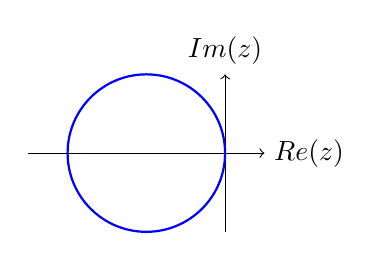
\begin{tikzpicture}
        \draw[->] (-2.5,0) -- (.5,0) node[right] {$\text{Re}(z)$};
        \draw[->] (0,-1) -- (0,1) node[above] {$\text{Im}(z)$};
        \draw[thick, blue] (-1,0) circle(1);
    \end{tikzpicture}$$
    Falta decidir si la regi\'on de estabilidad es el interior o el exterior de la circunferencia. Para ello, tomamos un punto de prueba, por ejemplo $z=-1$, y vemos que $|R(-1)| = 0 < 1$, por lo que el interior de la circunferencia pertenece a la regi\'on de estabilidad. 
    
    Por tanto, la regi\'on de estabilidad del m\'etodo de Euler expl\'icito es el interior de la circunferencia.
\end{ejem}

\section{Definiciones de estabilidad}

\begin{enumerate}[\bfseries 1.]
    \item \textbf{$A$-estabilidad ($A$-stability)}
    
    Un método numérico para ecuaciones diferenciales ordinarias se dice \textbf{$A$-estable} si su región de estabilidad absoluta $\mathcal{R}$ contiene a todo el semiplano izquierdo complejo:
    \[
    \mathcal{R} = \{ z \in \mathbb{C} : |R(z)| \le 1 \} \supseteq \{ z \in \mathbb{C} : \text{Re}(z) \le 0 \}
    \]
    
    \begin{itemize}
        \item \textbf{Significado práctico:} Al aplicarlo a la ecuación de prueba $y' = \lambda y$ con $\text{Re}(\lambda) < 0$, la solución numérica satisface:
        \[
        \lim_{n \to \infty} y_n = 0
        \]
        para cualquier tamaño de paso $h > 0$ (es decir, $h_{\max} = \infty$).
    \end{itemize}

    \vspace{0.5cm}

    \item \textbf{$L$-estabilidad ($L$-stability)}
    
    Un método numérico se dice \textbf{$L$-estable} si satisface dos condiciones:
    \begin{enumerate}[i)]
        \item Es $A$-estable.
        \item Su función de estabilidad $R(z)$ cumple:
        \[
        \lim_{\text{Re}(z) \to -\infty} R(z) = 0
        \]
    \end{enumerate}

    \begin{itemize}
        \item \textbf{Significado práctico:} Además de ser incondicionalmente estable, amortigua de forma inmediata las componentes extremadamente rígidas (\textit{stiff}, donde $\text{Re}(h\lambda) \to -\infty$) en un solo paso.
        \item \textbf{Ejemplo comparativo:}
        \begin{itemize}
            \item La \textbf{Regla del Trapecio} es $A$-estable pero \textbf{no} $L$-estable, pues:
            \[
            \lim_{z \to -\infty} R(z) = \lim_{z \to -\infty} \frac{2+z}{2-z} = -1
            \]
            (mantiene oscilaciones no amortiguadas de alta frecuencia).
            \item El método \textbf{SDIRK2} o \textbf{Euler Implícito} sí son $L$-estables, pues:
            \[
            \lim_{z \to -\infty} R(z) = \lim_{z \to -\infty} \frac{1}{1-z} = 0
            \]
        \end{itemize}
    \end{itemize}
\end{enumerate}
\vfill
\newpage